\chapter{Derivatives}\section{General}

\begin{enumerate}

\item  An equation like $$\sin ^2 x + \cos ^2 x = 1$$ is an identity because it is true for all values of $x$.  An equation like $$2x + 5 \cos x = 1$$ is not an identity because it is only true for specific values of $x$.  If you start with an identity and differentiate both sides, the result is also an identity; if you start with an equation that is not an identity and differentiate, the result is often not an identity.  (Try this on $\sin ^2 x + \cos ^2 x = 1$ and $2x + 5 \cos x = 1$.)
 Differentiate the following to show that the results are identities.   \cite{FWG}
\begin{enumerate} 

\item  $$\sin 2x = 2\sin x\cos x$$ 

\item   $$\cos 2x = \cos ^2 x - \sin ^2 x$$ \end{enumerate}


\item  Compare and contract explicit functions and implicit functions.

\item  Compare and contrast prime notation and Leibniz notation.

\item  Compare and contrast the meaning and usage of $$f'(c)$$ and $$f'(x).$$

\item  Certain values for a differentiable function are given in the following table.  Approximate the value of $f'(0.3).$  Explain how you found this approximation and why it is only an approximation.  (Maybe sketching a graph will help).
$$\begin{array}{|c|c|c|c|c|c|c|c|c|c|}\hline  x & 0.0 & 0.1 & 0.2 & 0.3 & 0.4 & 0.5 & 0.6 & 0.7 & 0.8  \cr \hline  f(x) & 5.0 & 4.1 & 4.0 & 4.6 & 5.5 & 6.2 & 6.5 & 6.1 & 5.7  \cr \hline  \end{array}$$

\item  Explain what an independent variable and a dependent variable are.  In an explicit function, how can we identify the assumed independent variable?  Why do we need to be told which is which in an implicit function?  In a graph, how do we identify the assumed independent variable?  If we are given a set of points or a table of ordered pairs, how do we identify the assumed independent variable?

\item  I did the 36 derivatives in the review at the end of the chapter.  I copied the original problem, found the derivative, and simplified.  This took me an average 1.25 minutes per derivative.  Let's assume a first-year Calculus student 4 times as long to complete the same exercises.  Set aside a time a do as many of these derivatives as you can.  If you run into one that you cannot do right away, mark it and go on.  When you are done, check the time and your work.  If it took you more than 5 minutes times the number you got correct including simplifying, then you need to practice more before the exam. 
 To turn in, analyze the derivatives you could not do right away and the ones you got wrong.  Also, talk about the amount of time it took you to do these problems.  Look at the list of derivative techniques in the review material and decide what you know well and what you have problems with.  What do you plan to do about this?

\item  Investigate the validity of this statement:   If $f(x) \le x$, then $f'(x) \le 1.$

\item  Look back at the homework and writing assignments you have done so far and identify concepts that you feel you know the best.  Identify areas that you need to improve on before the exam.  If you could improve on one concept before the exam, what concept would be the most beneficial to you and why? Which are the trickiest?

\item  We have seen $${{d\left( {f + g} \right)} \over {dx}} = {{df} \over {dx}} + {{dg} \over {dx}}$$ but $${{d\left( {f \cdot g} \right)} \over {dx}} \ne {{df} \over {dx}} \cdot {{dg} \over {dx}}.$$  Differentiation does not ``distribute'' across multiplication.  Make a list of operations that ``distribute'' across addition and some that do not with counterexamples to justify your choices.

\item  Write up to 5 distinct questions from the material in this chapter that I might ask on an exam about the following information:  $${{dy} \over {dx}} = {{dy} \over {du}} \cdot {{dy} \over {dx}}.$$

\item  Write up to 5 distinct questions from the material in this chapter that I might ask on an exam about the following information:  differentiability.

\item  Write up to 5 distinct questions from the material in this chapter that I might ask on an exam about the following information:  $f(x) = 3e^{2x}$ at $x = 0$.

\item  Write up to 5 distinct questions from the material in this chapter that I might ask on an exam about Figure \ref{Chapter3Figurea}. %Figure goes here

\begin{figure}[ht]
	\centering
		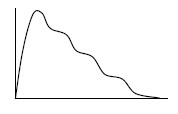
\includegraphics{TeXGraphics/Chapter3Fig.jpg}
	\caption{A graph}
	\label{Chapter3Figurea}
\end{figure}

\item  A differential helps us measure a function's sensitivity to change.  Suppose that we make a fixed small change in x, i.e., $dx$ is small and fixed.  If a small change in $x$ results in a large change in $y$, then we say the function is sensitive to change.  Since the differential gives us an approximate value for the change in $y$, then the differential also measures the sensitivity of the function. \begin{enumerate}


\item  Is $f(x) = x^3 - x$ more sensitive to small changes at $x = 0.5$, $x = 1$ or $x = 1.5$?  Explain what this means.


\item  Is $f(x) = x^2$ more sensitive to small changes than $f(x) = x^3$ is at $x = 1$?  Explain what this means.


\item  How can we quickly determine where a function is more sensitive  to change based on the graph of the derivative of the function? \end{enumerate}

\item  Explain the difference between $${{d^2 y} \over {dx^2 }}$$ and $$\left( {{{dy} \over {dx}}} \right)^2 .$$\end{enumerate}\section{Differentiability}\begin{enumerate}

\item  Compare and contrast differentiability and continuity.

\item  Describe geometrically when a function typically does not have a derivative at a point.   \cite{FWG}

\item  First, explain why $$\sqrt {x^2 }  = \left| x \right|.$$  At first glance it would appear that $$g(x) = \sqrt {x^2 } $$ is differentiable for all $x$, but we know $$f(x) = \left| x \right|$$ is not differentiable at $x = 0$.  Explain this ``paradox''.

\item  How are differentiability and continuity related?   \cite{FWG}

\item  What does it mean for a function to be differentiable?  Give three distinctly different sketches of functions that are not differentiable at particular points (make sure you indicate the point) and explain why each is not differentiable.

\item  Consider the graph of $$f(x) = \left| {\sin x} \right|.$$  Is this graph continuous?  If not, why not and where?  Is this graph differentiable?  If not, why not and where? \end{enumerate}\section{Tangent Lines}\begin{enumerate}

\item  For what values of $a$ and $b$ is $2x + y = b$ tangent to $y = ax^2$ at $x = 2$?  

\item  The line $L$ is tangent to the graph of the differentiable function $y = f(x)$ at the point (5, 2).  $L$ intersects the $y$-axis at (0, 4).  Find $f'(5).$  Provide an illustration along with the writing.

\item  What does it mean for a line to be tangent to a curve $C$ at a point $P$?   \cite{FWG}

\item  What is the relationship between secant lines and tangent lines?

\item  A friend says that if a straight line touches a curve at exactly one point, then it is tangent to the curve at that point. Your friend also says that if a straight line touches a curve at more than one point, then it cannot be tangent to the curve at any of those points.  What do you think?

 \end{enumerate}\section{Methods of Differentiation}\begin{enumerate}

\item  Compare and contrast the evaluation of the derivatives of the following functions.
\begin{enumerate}

\item  $y = 3^3$ 

\item   $y = x^3$ 

\item  $y = x^x$ 

\item   $y = 3^x$\end{enumerate}

\item  A friend of yours says that since the derivative of $f(x) = x^2 - 4x$ at $x = 2$ is 0 that means that $f(x) = x^2 - 4x$ is a constant function.  Help your friend understand this better.

\item  A student was absent from class today and asked you to help him understand when and how to use logarithmic differentiation.  Give him several examples that do not need logarithmic differentiation and several that do.  Explain the process.

\item  A student was absent from class yesterday and asked you to help him understand the chain rule.  In particular, he needs help understanding how to find the derivatives of $\sin 5 x$ and $\sin x^5$.  Explain this to him.

\item  As a mathematical quiz show contestant, you are asked to find the value $$F'\left( 7 \right)$$ for the composition $$F = f \circ g.$$  The functions $f$ and $g$ are unknown, but you are permitted to ask exactly 3 questions to help you find the answer.  What 3 questions should you ask?  \cite{EP}

\item  Compare and contrast the evaluation of the derivatives of $$e^{x\sin x} ,$$ $$e^x \sin x$$ and $$xe^{\sin x} .$$

\item  Compare and contrast the product and the quotient rules.

\item  Create a concept map of the derivatives of the trigonometric functions that emphasizes the symmetry and patterns of the derivatives.  Describe these patterns in words. 

\item  Create some new derivative rules based on the rules we have learned so far.  First, if $$y = {1 \over u},$$ what is $${{dy} \over {dx}}?$$  This would be called the Reciprocal Rule.  Also, if $y = uvw$, what is $${{dy} \over {dx}}?$$  This is the Triple Product Rule.  What would the Quadruple Rule be?  

\item  Derive a general formula for the derivative of $$y = f(x)^{g(x)} .$$  Make comparisons to the rules for the derivatives of $$u = a^{g(x)} $$ and $$v = f(x)^b .$$

\item  Each time we use implicit differentiation we are able to rewrite the resulting equation in the form $$f(x,y) = y' \cdot g(x,y)$$ for some expressions $f$ and $g$.  Explain why this can always be done; that is, why doesn't the chain rule ever produce a term like $$(y')^2 $$ or $${1 \over {y'}}?  \ \cite{SM}$$   

\item  Explain how to derive the derivative formula for $$y = \sin ^{ - 1} x.$$

\item  Explain what needs to be true about a function for you to need the chain rule?  Give examples of functions that need the chain rule and functions that do not need the chain rule.  Be as inclusive as possible.

\item  Many students prefer the product rule to the quotient rule.  Explain how each can be used to find the derivative of $$f(x) = {{\left( {2x - 3} \right)^4 } \over {\left( {x - 1} \right)^3 }}.$$  Which do you prefer and why?

\item  Once you know the derivatives of $\sin x$ and $\cos x$, how can you find the derivatives of 
$\tan x$, $\cot x$, $\sec x$, and $\csc x$?   Choose an example to annotate.   \cite{FWG}

\item  Suppose $$F(x) = f\left( {g\left( {h(x)} \right)} \right).$$  Write out the chain rule for $$F'\left( x \right).$$  What numerical values would be needed to find $$F'\left( 7 \right)? \ \cite{EP}$$    Write out the chain rule for $$G(x) = f\left( {g\left( {h\left( {m\left( x \right)} \right)} \right)} \right).$$ What numerical values would be needed to find $$G'\left( 2 \right)?$$

\item  Using that $$\left( {\sin x} \right)^\prime   = \cos x$$ and $$\left( {\cos x} \right)^\prime   =  - \sin x,$$ derive the formulas for $\tan x$, $\cot x$, $\sec x$, and $\csc x$.  When we take the derivative of $\cos x$, the sign of the result is opposite of the original.  Also, note that $\tan x$, $\cot x$, and $\csc x$ have $\cos x$ in their definitions.  Which of the derivatives result in a change of sign?  Why don't all of the derivatives of the trigonometric functions with $\cos x$ in their definition result in a change of sign?  Develop a mnemonic to help you remember these rules. 

\item  We can find the derivative of certain exponential functions without the chain rule.  Compare and contrast calculating the derivative of $$f(x) = e^{2x} $$ using the chain rule and using the product rule on $$f(x) = e^{2x}  = \left( {e^x } \right)\left( {e^x } \right).$$  Do the same with $$f(x) = e^{3x} .$$

\item  We usually talk about trigonometric functions in pairs.  Cosine is paired with sine, tangent is paired with secant and cotangent is paired with cosecant.  Describe a trigonometric relationship and a calculus relationship to justify each pairing.

\item  You and a friend compared answers to your homework.  Your friend found the derivative of $$p = {{\tan t} \over {1 + \tan t}}$$ and got $${{dp} \over {dt}} = {1 \over {1 + \sin 2t}}$$ which doesn't look anything like your answer.  If you are both right, explain how each of you got the answer and why they are the same.  If one of you is wrong, explain the error and how to avoid it in the future.

\item  You found the derivative of $$M(x) = {{2x - 3} \over {x^3 }}$$ and got $$M'(x) = {{9 - 4x} \over {x^4 }}.$$  You decided to check your answer with a friend's answer and she got $$M'(x) =  - 4x^{ - 3}  + 9x^{ - 4} .$$  Should either of you be worried?  Which answer is ``better''?  

\item  You have been cautioned against multiplying out the terms of a derivative.  Explain why having a factored form of $$f'\left( x \right)$$ is helpful.  How close does the product rule bring you to a nicely factored form of $$f'\left( x \right)? \  \cite{SM}
$$  
\item  A friend of yours has the following work on their paper.
 $$\displaylines{  f(x) = x^{ - {3 \mathord{\left/ {\vphantom {3 2}} \right. \kern-\nulldelimiterspace} 2}}  \cr   f'(x) =  - {{3x^{ - {1 \mathord{\left/ {\vphantom {1 2}} \right. \kern-\nulldelimiterspace} 2}} } \over 2} \cr} $$
Gently and correctly help your friend understand the mistake he made and give him advice about how to avoid this mistake in the future.

\item  A friend of yours has the following work on their paper.
 $$\displaylines{  f(x) = {{\sin x} \over x} \cr   f'(x) = 1 \cr} $$
Why do you think your friend made this mistake?  Gently and correctly help your friend understand the mistake he made and give him advice about how to avoid this mistake in the future.

\item  Compare and contrast the evaluation of the derivatives of $$\sin ^2 x$$ and $$\sin x^2 .$$

\item  Compare and contrast the evaluation of the derivatives of $${{x^3  - 1} \over {x^2 }}$$ and $${{x^2 } \over {x^3  - 1}}.$$

\item  Consider the relationship $x^2 + y^2 = 100$ where $y < 0$.  Use implicit differentiation to find $${{dy} \over {dx}}.$$  Now, solve for $y$ and find $${{dy} \over {dx}}$$ in the usual way.  Show that the results are the same.  Would the results be the same if we did not restrict y to be negative?  Why do we need implicit differentiation?

\item  Using the definition of 
$$\left| a \right| = \left\{ \begin{array}{ll} a, & \,a \ge 0 \cr    - a, & \,a < 0 \cr \end{array} \right.,$$ write a piecewise definition of $$y = \ln \left| x \right|.$$  Now, find $$y'.$$  Observations? 

\end{enumerate}\section{Graphs and the Derivative}\begin{enumerate}

\item  Consider the function $f(x)$, its vertical translation $g(x) = f(x) + a$, and its horizontal translation $h(x) = f(x + a)$.  How do the derivatives of $g$ and $h$ compare to the derivative of $f$?  Explain how the graphs of the function and its translations confirm your analytic results.

\item  Consider the graph of $y = f'(x)$ in Figure \ref{Chapter3a}.  Of the 5 points marked on the graph, choose and label the point where $f(x)$ is the largest. Of the 5 points marked on the graph, choose and label the point where $f(x)$ is the smallest.  Can you approximate those values of $f(x)$?  Explain why you made the choices you did.   %put figure 1 here

\begin{figure}[ht]
	\centering
		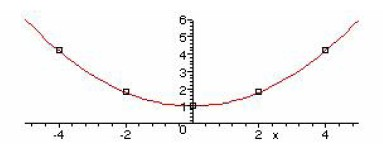
\includegraphics{TeXGraphics/Chapter3a.jpg}
	\caption{Approximating derivatives}
	\label{Chapter3a}
\end{figure}




\item  Consider the graph of $y = f(x)$ in Figure \ref{derivativegraph}.  Create axes and scales for this graph.  Mark and label on the graph the point at which $f'(x)$ has the greatest positive value,  the point at which $f'(x)$ has the smallest absolute value and the point at which $f'(x)$ has the greatest negative value.  Approximate those values?  Explain your work.                       %put DerivativeFunction.jpg here
\begin{figure}[ht]
	\centering
		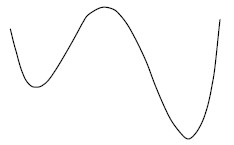
\includegraphics{TeXGraphics/DerivativeFunction.jpg}
	\caption{Extreme derivatives}
	\label{derivativegraph}
\end{figure}


\item  Does the curve $y = x^3$ ever have a negative slope?  If so, where?  If not, justify your answer.  What does this say about the shape of the curve?

\item  Find the angle between the circle $x^2 + y^2 = 1$ and the circle $x^2 + (y - 1)^2 = 1$ at each of the two points of intersection.

\item  How does the graph of $-f(x)$ compare to the graph of $f(x)$?  How does the value of $ - f'(a)$ compare to $f'(a)?$   How does the graph of $3f(x)$ compare to the graph of $f(x)$?  How does the value of $3f'(a)$ compare to $f'(a)?$  Be sure to talk about the connection between the derivative and slope.

\item  Investigate the validity of this statement:  If the derivative of a function is positive in a given interval, then the function is increasing.

\item  Use graphical analysis to argue that the derivative of $\cos x$ is $-\sin x$.   \cite{SM}

\item  Investigate the validity of this statement:  If $f(p)$ and $f(q)$ are both absolute minimum values of $f$ on its domain, then $f(p) = f(q)$.   \cite{EP}

\item  Investigate the validity of this statement:  Relative minima can occur at many different locations, but the absolute minimum can only occur at one location.

\item  Investigate the validity of this statement:  Every local extreme of the function $f$ occurs at a point where $$f'(x) = 0.$$  Does the answer change if we replace the word ``local'' with ``global''?

 \end{enumerate}\section{Applications of the Derivative}\begin{enumerate}

\item  A friend of yours missed the first day we talked about related rates problems and wants to know what we did so he can complete the homework.  Rewrite and improve Example 1 from this section of the test to help explain the process to him.  

\item  A linear approximation to $f$ at $x_0$ is a line $L(x) = ax + b$ where $$L\left( {x_0 } \right) = f\left( {x_0 } \right)$$ and $$L'\left( {x_0 } \right) = f'\left( {x_0 } \right).$$  What if we wanted to approximate the curve with a parabola instead of a line.  Consider the quadratic function $$Q\left( x \right) = ax^2  + bx + c$$ and the curve $$f\left( x \right) = \left( {1 - x} \right)^{ - 1} $$ and the point $$x_0  = 0.$$  Find the coefficients $a$, $b$ and $c$ so that $$Q\left( {x_0 } \right) = f\left( {x_0 } \right),$$ $$Q'\left( {x_0 } \right) = f'\left( {x_0 } \right),$$ and $$Q''\left( {x_0 } \right) = f''\left( {x_0 } \right).$$  Graph $f$ and $Q$.  Zoom in on the point $$x_0  = 0.$$  Comment on what you see. If the results of the graph are not as expected, then something is amiss.  How does this quadratic approximation compare to a linear approximation?

\item  Choose a specific related rates problem and use dimensional analysis to show that the units work out correctly.

\item  Compare and contract implicit differentiation and differentiation in related rates problems.

\item  Compare and contrast rectilinear motion problems and related rates problems.

\item  Compare and contrast the concepts of position, distance, and displacement within the scope of rectilinear motion.

\item  Consider a general linear function $L(x) = ax + b$.  Show that if $L$ is a linearization of $f$ at $x_0$, then $$L\left( {x_0 } \right) = f\left( {x_0 } \right)$$ and $$L'\left( {x_0 } \right) = f'\left( {x_0 } \right).$$  Explain why this must be true.

\item  Describe a situation that can be solved using related rates methods.  Explain what is happening to each variable and each rate at a specific time.  How would looking at the same situation at a different time impact the variables and rates?

\item  Discuss error propagation, including relative error, and percentage error.   \cite{SBS}

\item  How do derivatives arise in the study of motion?  What can you learn about a body's motion along a line by examining the derivatives of the body's position function?   \cite{FWG}

\item  How do related rate problems arise?   \cite{FWG}

\item  If you are doing a related rates problem and you find that one of the dependent variables is constant, what happens?  Using an example of your own choice show that it doesn't matter whether you know the variable is constant before you start or later in the problem.

\item  Linearization can give us ``good'' approximations or ``bad'' approximations.  Explain why it can be said that $y = x$ is a good approximation to $y = \sin x$ near $x = 0$ but $y = 1$ is not a good approximation to $y = \cos x$ near $x = 0$.   \cite{SM}

\item  Tangent line approximations are useful only if $\Delta x$ is small.  Consider the approximation of $$y = \sqrt x $$ only using the linearization of $$y = \sqrt x $$ at the point $x = 81$.  Make a table of values of approximations and actual values of $$y = \sqrt x $$ for various values of $x$ around $x = 81$.  What other calculations might you make?  What values would be good to have in your table (I can think of several)?  Discuss your observations.

\item  The equations for free fall at the surfaces of Vulcan and Kronos are $s = 1.86t^2$ meters and $s = 11.44t^2$ meters, respectively, where $t$ is time in seconds.  How long does it take a rock falling from rest to reach a velocity of 27.8 m/sec on each planet?  Which planet has ``stronger'' gravity?  How can you determine that from the equations and/or graphs alone?

\item  Using the definition of the derivative, explain why the units of velocity are distance/time and why the units of acceleration are ${\rm{distance}}/({\rm{time}})^2$.

\item  What is a differential?  What is it used for?  What are the notational alternatives to using a differential and why, in some cases, is a differential an advantage over the alternative?

\item  What is the difference between speed and velocity?  We use both of these words in our every day language, but one of them we usually use incorrectly.  Which one is it?  What does acceleration mean in terms of speed?  Why do we call the accelerator the accelerator in our car?  Is it always used as an accelerator in the mathematical sense of the word?  How else does acceleration happen when we are driving a car?

\item  What is the function that gives the height of an object shot straight up from the ground at an initial velocity of 30 feet/sec?  Graph this function.  Find the  velocity and acceleration functions and graph them, too.  Identify the important features of the graphs and describe what is happening at those points.  Explain why the acceleration function looks the way it does.  (What would it say about the Earth if the acceleration function looked different than it does?  Have you ever seen the movie Hypercube?)

\item  When we differentiate with respect to $t$ for related rates, we can use any form of the equation as long as we keep note the domain.  For example, differentiate $$d = \sqrt {x^2  + y^2 } $$ with respect to $t$.  Now, conveniently change the equation and differentiate again.  Show that the 2 results are the same thing.  How could this be useful when using related rates?

\item  For rectilinear motion we use a function and its first and second derivatives.  What information do we obtain from the original function and what types of questions can we answer with it?  The first derivative?  The second derivative?

\item  Why is it important to identify the independent variable before finding a derivative?  What is the independent variable in a related rates problem?  How does this impact how we solve a related rates problem?  
\end{enumerate}\section{Higher Order Derivatives}\begin{enumerate}

\item  Find constants $A$, $B$, and $C$ so that $$y = Ax^3  + Bx + C$$ satisfies the equation $$y''' + 2y'' - 3y' + y = x.$$  

\item  Find the derivative of $y = \sin x$ of many different orders.  From this data, determine an algorithm for finding any derivative of $y = \sin x$.  Explain your algorithm so others can use it.  Find $${{d^{123} y} \over {dx^{123} }}.$$  Find $${{d^{708} y} \over {dx^{708} }}.$$

\item  What is a second derivative?  A third derivative?  How many derivatives do the functions you know have?   \cite{FWG}

\item  Consider a polynomial of degree $n$.  Describe as fully as possible, all the derivatives of this polynomial of any order.
\end{enumerate}
